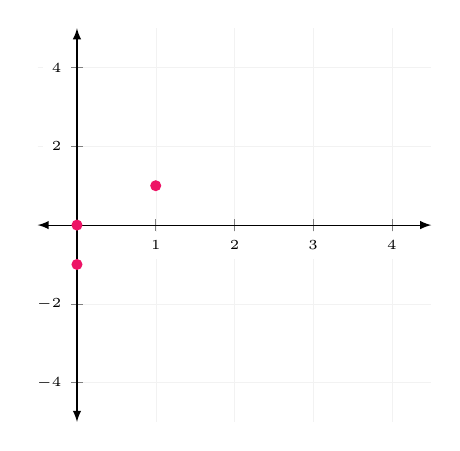
\begin{tikzpicture}[baseline = (current bounding box.north)]
					\begin{axis}[
						anchor=origin,
						disabledatascaling,
						xmin=0,xmax=4,
						ymin=-4,ymax=4,
						xtick={0,...,4},
						ytick={-4,-2,0,2,4},
						x=1cm,y=0.5cm,
						grid=both,
						grid style={line width=.1pt, draw=gray!10},
						axis lines=middle,
						minor tick num=0,
						enlarge x limits={abs=0.5},
						enlarge y limits={abs=1.0},
						axis line style={latex-latex},
						ticklabel style={font=\tiny,fill=white},
						xlabel style={at={(ticklabel* cs:1)},anchor=north west},
						ylabel style={at={(ticklabel* cs:1)},anchor=south west}
					]
						\fill [WildStrawberry] (1,1) circle[radius=2pt];
						\fill [WildStrawberry] (0,-1) circle[radius=2pt];
						\fill [WildStrawberry] (0,0) circle[radius=2pt];
					\end{axis}
				\end{tikzpicture}
